\documentclass{article}

\usepackage{bnaic}
\usepackage{graphicx}
\usepackage{mathtools}
\usepackage{amsmath}
\usepackage{caption}
\usepackage{subcaption}
\usepackage{comment}

\usepackage[x11names,rgb,table]{xcolor}
\usepackage{tikz}
\usepackage{pgfplots}
%\pgfplotsset{compat=newest}
\usetikzlibrary{arrows,shapes,petri}
\usepackage{gnuplot-lua-tikz}

\newcommand{\eg}{{\it e.g.,}~}
\newcommand{\ie}{{\it i.e.,}~}
\newcommand{\argmax}{\operatornamewithlimits{argmax}}

\newcommand{\coolalg}{\textsc{mcms}}
\newcommand{\coolalglong}{Monte Carlo *-Minimax Search}
\newcommand{\mcms}{\textsc{mcms}}
\newcommand{\mcts}{\textsc{mcts}}
\newcommand{\bmcts}{\textsc{mcts*}}
%\newcommand{\expectiminimax}{\textsc{Expectimax}}
\newcommand{\expectimax}{\textsc{expectimax}}
\newcommand{\dpw}{\textsc{dpw}}
\newcommand{\expecti}{exp}
\newcommand{\expss}{exp\textsc{ss}}
\newcommand{\starone}{Star1}
\newcommand{\startwo}{Star2}
%\newcommand{\staroness}{s1\textsc{ss}}
%\newcommand{\startwoss}{s2\textsc{ss}}
\newcommand{\staroness}{star1\textsc{ss}}
\newcommand{\startwoss}{star2\textsc{ss}}
\newcommand{\pig}{Pig}
\newcommand{\cant}{Can't Stop}
\newcommand{\ra}{Ra}
\newcommand{\ewn}{\textsc{ewn}}
\newcommand{\playername}[1]{\emph{#1}}


% ML Jun24: These comments are 
%\section{The bnaic Package}
%The \verb+bnaic.sty+ file is a package that is to be used together with
%the standard \verb+article+ document class. Please adhere strictly to the instructions of this document. The bnaic style file uses the standard \verb+times+ package and the \verb+geometry+ package, which is included in the bnaic package; please do not change it! 

%% if your are not using LaTeX2e use instead
%% \documentstyle[bnaic]{article}

%% begin document with title, author and affiliations


% ML Jun24: These comments are from the BNAIC author instructions

%The title of the article has to appear in bold and the \verb+\huge+ keyword has to be used to set the correct font size. For
%the authors and their affiliations, three cases are distinguished:

%\begin{itemize}
%\item One author: define the author with \verb+\author+ and the affiliation
%   with \verb+\date+.
%\item Multiple authors, all with the same affiliation: define the authors with
%   \verb+\author+, separated by \verb+\and+, and the affiliation with
%   \verb+\date+.
%\item Multiple authors, multiple affiliations: define the
%   authors with \verb+\author+. Put after each name a letter for the
%   affiliation, generated by \verb+\affila+, \verb+\affilb+, etc. On the
%   next lines: one affiliation per line, each preceded by the appropriate letter
%   generated by \verb+\affila+, \verb+\affilb+. See the title of this document.
%\end{itemize}

%Note that affiliations have to appear in italics.

\title{\textbf{\huge Monte Carlo *-Minimax Search\footnotemark[1]}}
\author{Marc Lanctot\affila \and
        Abdallah Saffidine\affilb \and
        Joel Veness\affilc \and
        Chris Archibald\affilc \and 
        Mark H.M. Winands\affila}
\date{\small \affila\ \textit{Department of Knowledge Engineering, Maastricht University}\\
      \affilb\ \textit{LAMSADE, Universit\'{e} Paris-Dauphine, France}\\
      \affilc\ \textit{Department of Computing Science, University of Alberta, Canada}}
%\date{\affila\ \textit{Department of Knowledge Engineering, Maastricht University,\\ P.O. Box 616, 6200 MD Maastricht, The Netherlands}}
%    \affilb\ \textit{The Company Ltd. P.O.Box 4321 Antwerp}}

\pagestyle{empty}

\begin{document}
\ttl
\thispagestyle{empty}


% ML Jun24: From author instructions:
%\section{The abstract}
%Put the abstract before the first section with the \verb+abstract+
%environment. Please start the first paragraph of your abstract with a \verb+\noindent+ command.

\begin{abstract}
\noindent   This paper presents an overview of Monte Carlo *-Minimax Search (MCMS), a Monte Carlo search algorithm for 
  turned-based, stochastic, two-player, zero-sum games of perfect information.
  MCMS combines sparse sampling techniques used in MDP planning with classic pruning techniques developed 
  for adversarial expectimax planning.
  MCMS has been compared to the traditional *-Minimax approaches, as well as MCTS  
  on four games. Results show that MCMS can be compete with enhanced MCTS variants in some domains, 
  while outperforming the equivalent classic approaches given the same search time. 
\end{abstract}

\footnotetext[1]{The full version of this paper has been accepted for 23rd Joint Conference on Artificial Intelligence (IJCAI 2013).}

\section{Introduction}

Monte Carlo sampling in game-tree search has received much attention in recent years due to successful application to 
Go-playing programs. 
While the community has focused mainly on deterministic two-player games, such as Go, Hex, and Lines of Action, there
has been a growing interest in studying these sample-based approaches outside this traditional setting. The class of 
perfect information games with chance events-- which includes, for example, Backgammon-- has received comparatively 
little attention. 

Classic algorithms such as minimax perform a depth-limited search from the root (current position), 
returning a heuristic value if the depth limit is reached, or the value of the best available move otherwise.  
$\alpha \beta$ pruning prevents searching provably wasteful portions of the tree. The largest 
and most famous application of these techniques was in IBM's Deep Blue chess program which defeated the human world 
champion. Expectimax is an extension of minimax that will return the expected values over children at 
chance nodes. The *-minimax algorithm extends $\alpha \beta$ pruning to perfect information games with 
chance nodes~\cite{Ballard83}. 

\section{Sparse Sampling in *-Minimax Search}

Monte Carlo *-Minimax Search (MCMS) samples a subset of the chance event outcomes at chance nodes
during its search. In essence, the algorithm applies *-minimax (Star1 or Star2) search to a sampled 
and significantly smaller subgame to effectively increase the depth reached in a fixed time limit. 
This way of using sampling to reduce computation is inspired by sparse sampling methods from the 
MDP planning literature~\cite{kearns99} and is in contrast with recent Monte Carlo search algorithms such as Monte 
Carlo Tree Search (MCTS)~\cite{Coulom07Efficient}, which are simulation-based and build a model of 
the game tree incrementally.

Consider Figure~\ref{fig:example}. Suppose the number of chance event outcomes is $N$. 
For example, in a game where players roll two six-sided dice, it may be that $N = 36$.  
Suppose the algorithm returns a value of $v_i$ for the subtree below outcome $i$, and the probability of outcome
$i$ is $p_i$. Expectimax and *-Minimax will return the weighted sum $\sum_{i = 1}^N v_i p_i$. MCMS, however, 
first samples $c < N$ outcomes (with replacement), sets $p'_i = 1/c$ and returns $\sum_{i = 1}^c p'_i v'_i$, 
where $v'_i$ is the value that MCMS returns for the subtree under outcome $i$. 

\begin{figure}[t!]
        \centering
        %\begin{subfigure}[m]{0.32\textwidth}
        \begin{subfigure}[m]{0.4\textwidth}
                \centering
                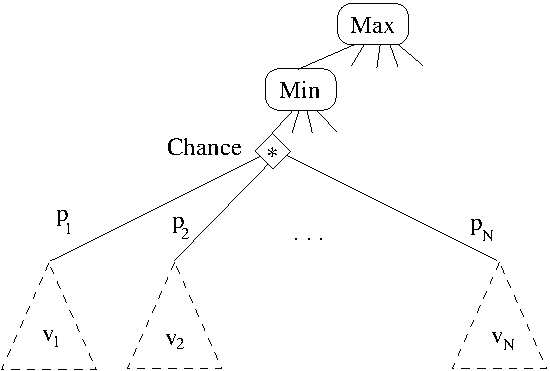
\includegraphics[width=\textwidth]{example}
                %\caption{A gull}
                %\label{fig:gull}
        \end{subfigure}%
        ~~~~~~~~~~~~ $\rightarrow$ ~~~~~~~~~~~~
        %add desired spacing between images, e. g. ~, \quad, \qquad etc.
          %(or a blank line to force the subfigure onto a new line)
        %\begin{subfigure}[m]{0.24\textwidth}
        \begin{subfigure}[m]{0.23\textwidth}
                \centering
                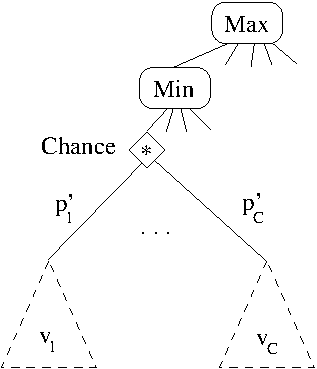
\includegraphics[width=\textwidth]{example2}
                %\caption{A tiger}
                %\label{fig:tiger}
        \end{subfigure}
        \caption{Example of sampling in MCMS.}\label{fig:example}
\end{figure}

\begin{figure*}[h]
\small
  \centering
  \hspace{-0.3cm} 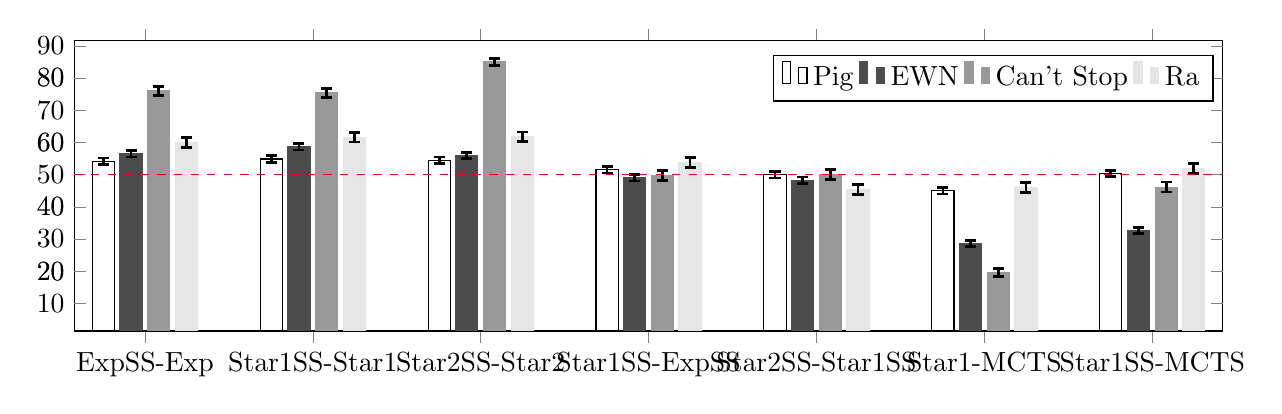
\begin{tikzpicture}
    \begin{axis}[
        ybar,
        ymin=7,
        enlargelimits=0.07,
        %width=535pt,
        width=460pt,
        height=150pt,
        bar width=8pt,
        extra y ticks={10,20,30,40,50,60,70,80,90},
        legend style={at={(0.8,0.95)},
          anchor=north,legend columns=-1},
        %ylabel={\#participants},
        symbolic x coords={ExpSS-Exp,Star1SS-Star1,Star2SS-Star2,Star1SS-ExpSS,Star2SS-Star1SS,Star1-MCTS,Star1SS-MCTS},
        xtick=data,
        %every node near coord/.style={font=\tiny},
        %nodes near coords,
        %nodes near coords align={vertical},
        %cycle list = {black,black!80,black!60,black!40,black!20},
        cycle list = {black,black!70,black!40,black!10},
      ]
      %pig
      \addplot+[error bars/.cd, y dir=both, y explicit, error bar style={line width=1pt, color=black}, error mark options={
          rotate=90,
          mark size=2pt,
          line width=1pt
      }] coordinates {
        (ExpSS-Exp,54.16) +- (0,0.98) 
        (Star1SS-Star1,54.85) +- (0,0.98) 
        (Star2SS-Star2,54.51) +- (0,0.98)
        (Star1SS-ExpSS,51.47) +- (0,0.98)
        (Star2SS-Star1SS,49.96) +- (0,0.98)
        (Star1-MCTS,44.9845) +- (0,0.98)
        (Star1SS-MCTS,50.37) +- (0,0.98)
      };
      % ewn
      \addplot+[fill, text = black, error bars/.cd, y dir=both, y explicit, error bar style={line width=1pt, color=black}, error mark options={
          rotate=90,
          mark size=2pt,
          line width=1pt
      }] coordinates {
        (ExpSS-Exp,56.45) +- (0,0.97) 
        (Star1SS-Star1,58.61) +- (0,0.97) 
        (Star2SS-Star2,55.97) +- (0,0.98)
        (Star1SS-ExpSS,49.03) +- (0,0.98)
        (Star2SS-Star1SS,48.31) +- (0,0.98)
        (Star1-MCTS,28.66) +- (0,0.89)
        (Star1SS-MCTS,32.56) +- (0,0.92)
      };
      % can't stop
      \addplot+[fill, text = black, error bars/.cd, y dir=both, y explicit, error bar style={line width=1pt, color=black}, error mark options={
          rotate=90,
          mark size=2pt,
          line width=1pt
      }] coordinates {
        (ExpSS-Exp,75.98) +- (0, 1.32) 
        (Star1SS-Star1,75.35) +- (0,1.34) 
        (Star2SS-Star2,85.03) +- (0,1.11)
        (Star1SS-ExpSS,49.63) +- (0,1.55)
        (Star2SS-Star1SS,50) +- (0,1.55)
        (Star1-MCTS,19.58) +- (0,1.23)
        (Star1SS-MCTS,46.13) +- (0,1.55)
      };
      % ra
      \addplot+[fill, text = black, error bars/.cd, y dir=both, y explicit, error bar style={line width=1pt, color=black}, error mark options={
          rotate=90,
          mark size=2pt,
          line width=1pt
      }] coordinates {
        (ExpSS-Exp,59.90) +- (0,1.56) 
        (Star1SS-Star1,61.63) +- (0,1.52) 
        (Star2SS-Star2,61.70) +- (0,1.52)
        (Star1SS-ExpSS,53.79) +- (0,1.56)
        (Star2SS-Star1SS,45.33) +- (0,1.55)
        (Star1-MCTS,46.09) +- (0,1.52)
        (Star1SS-MCTS,51.90) +- (0,1.56)
      };
      \draw [red,dashed] ({rel axis cs:0,0}|-{axis cs:ExpSS-Exp,50}) -- ({rel axis cs:1,0}|-{axis cs:ExpSS-Exp,50});
      %\addplot+[red,sharp plot,update limits=false] coordinates {(ExpSS-Exp,50.0) (MCTS-DPW,50.00)}; 
      %\addplot+[error bars/.cd, y dir=both, y explicit, error bar style={line width=1pt}, error mark options={
      %      rotate=90,
      %      %red,
      %      mark size=2pt,
      %      line width=1pt
      %    }] coordinates {(ExpSS/Exp,45.84) +- (0,0.98) (Star1SS/Star1,45.15) +- (0,0.98) (Star2SS/Star2,45.49) +- (0,0.98)};
      %\addplot coordinates {(tool8,4) (tool9,4) (tool10,4)};
      %\addplot coordinates {(tool8,1) (tool9,1) (tool10,1)};
      \legend{Pig,EWN,Can't Stop,Ra}
    \end{axis}
  \end{tikzpicture}
  \caption{Results of playing strength experiments.
    Each bar represents the percentage of wins for $p_{\text{\footnotesize left}}$ in a 
    $p_{\text{\footnotesize left}}$-$p_{\text{\footnotesize right}}$ pairing. 
    % ML-Apr19 Start
    (Positions are swapped and this notation refers only to the name order.)
    % ML-Apr19 End
    Errors bars represent 95\% confidence intervals. 
    Here, %the best variant of \mcts{} is used in each domain. 
    Exp refers to expectimax, $X$SS refers to algorithm $X$ with sparse sampling, and Star1 and Star2 represent two 
    different pruning variants of *-minimax.
    %\expecti{}-\mcts{}, \expss{}-\mcts{}, \startwo{}-\mcts{}, and \startwoss{}-\expss{} are intentionally omitted since they look similar to 
    %\starone{}-\mcts{}, \staroness{}-\mcts{}, \starone{}-\mcts{}, and \staroness{}-\expss{}, respectively. 
    %\expecti{}-\mcts{}, \expss{}-\mcts{}, \startwo{}-\mcts{}, and \startwoss{} are intentionally omitted since they look similar to \starone{}-\mcts{} and \staroness{}-\mcts{}.
    \label{fig:perf}}
\end{figure*}

\section{Results and Remarks}

In the full paper, we show that the value returned by MCMS approaches the value computed 
by *-Minimax as the sample width, $c$, increases. 
Furthermore, the convergence does not depend on the number of states. 
In practice, MCMS is shown to exhibit lower regret and bias than *-minimax on Pig. 
This comes at a cost of increased variance due to sampling. 
As seen in Figure~\ref{fig:perf} across four games: Pig, EinStein w\"{u}rfelt Nicht! (EWN), Can't Stop, and Ra.
show that MCMS (ExpSS, Star1SS, or Star2SS) 
consistently outperforms its classic counterpart (expectimax, Star1, or Star2). 
When playing against MCTS, MCMS wins 4-16\% more than *-minimax. 
MCMS is also competitive against state-of-the-art MCTS in two of the four chosen games, outperforming 
MCTS in Ra. 

\bibliographystyle{plain}
\bibliography{mcms-bnaic}



\end{document}








